\chapter{Other improvements}
\label{sec:other}
Besides team assignments and assignments mirroring, during the last year we worked on more concepts, such as assignment dashboard or improved submissions. The purpose of this chapter is to bring a brief overview about these other concepts.

\section{Peer review and improved submissions}

In the educational context, peer reviews were shown to improve the engagement with the others work, they provide a different type of feedback from a different point of view than the instructor’s one. Peer reviews foster discussion and experience exchange between the students, facilitating the social learning effect, a valued phenomenon according to the constructivist and constructionist learning theories. \cite{peerreview}


In this part of our work, we are describing implementation and flow of peer-review and improved submission support in Courses 2 learning management system. It is important to note, that support for peer reviews was already implemented in this system however it had to be refactored. Improved submissions were not present, however teacher could emulate them with creation of multiple assignments. Yet this approach was somehow confusing for students. One of the problems was, that there was a mess among submitted assignments and this problem needed to be fixed.


\subsection{Peer-review workflow}

The teacher creates the desired Assignment in the Assignments module. While creating an assignment the teacher can set its type (URL of FILE), deadlines, and allow improved submissions. The teacher may also enter questions for review phase if it is allowed. These will then be shown to other students.

\begin{figure}[h]
    \centering
    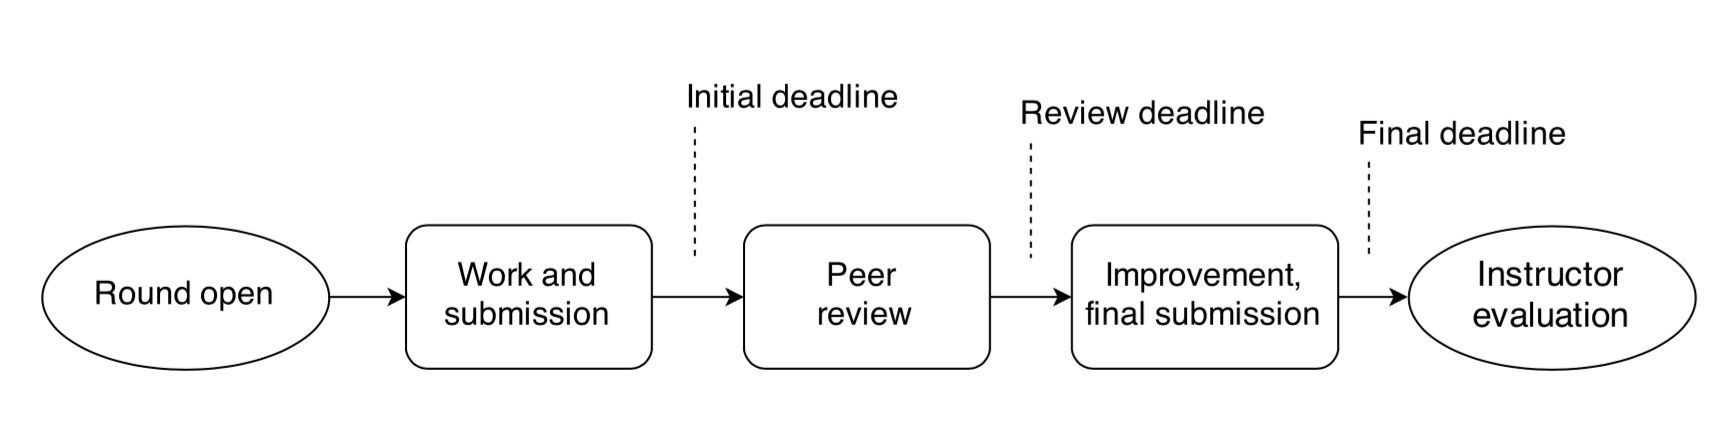
\includegraphics[width=\textwidth]{images/peerreview.png}
    \caption{Peer review and improved submission flow}
    \label{fig:improved_submissions}
\end{figure}

The workflow of a single assignment round is depicted at \ref{fig:improved_submissions}. First two parts are mandatory, while the other three are configurable. In the next section, we are going to describe full workflow of the round.


Once the round is open for submission by the course teacher, the students work on initial submission before the first deadline. Then, in second phase, the students who submitted their work are assigned three submissions to review (these submissions were submitted by their classmates and should be anonymouse - the reviewer does not know whose work is he assigned). These reviews should serve as feedback to their work and students should take them into account in the next phase. This is called improved submission, which is after all evaluated by the course teacher.


\section{Connection of Assignment and Note module}

One of the things, that students often complained was insufficient assignment description. In original Courses 2 assignments module there was just one simple textarea the teacher could enter description of any assignment. This problem needed to be solved.

First possible solution was to implement some assignments description submodule, but then again, we had already implemented Note module. It was easier and more usable to link output of this module to Assignments module.

\subsection{Note module}
Screenshot of Note module can be seen at figure \ref{courses2screen}. This module is providing two simple use cases.

For teacher, notes module is used to publish notes for lectures. Teacher can publish as many notes as he wants, each using HTML markup so it can include images, graphics, CSS styles and hyperlinks. These notes can also contain sub-notes.

As opposed to teachers, students can only view these notes. As the reallity showed, these notes ofted contained important recommendations or explanations which could help students to improve their submissions. So why not link them together, right?

\begin{figure}[h]
    \centering
    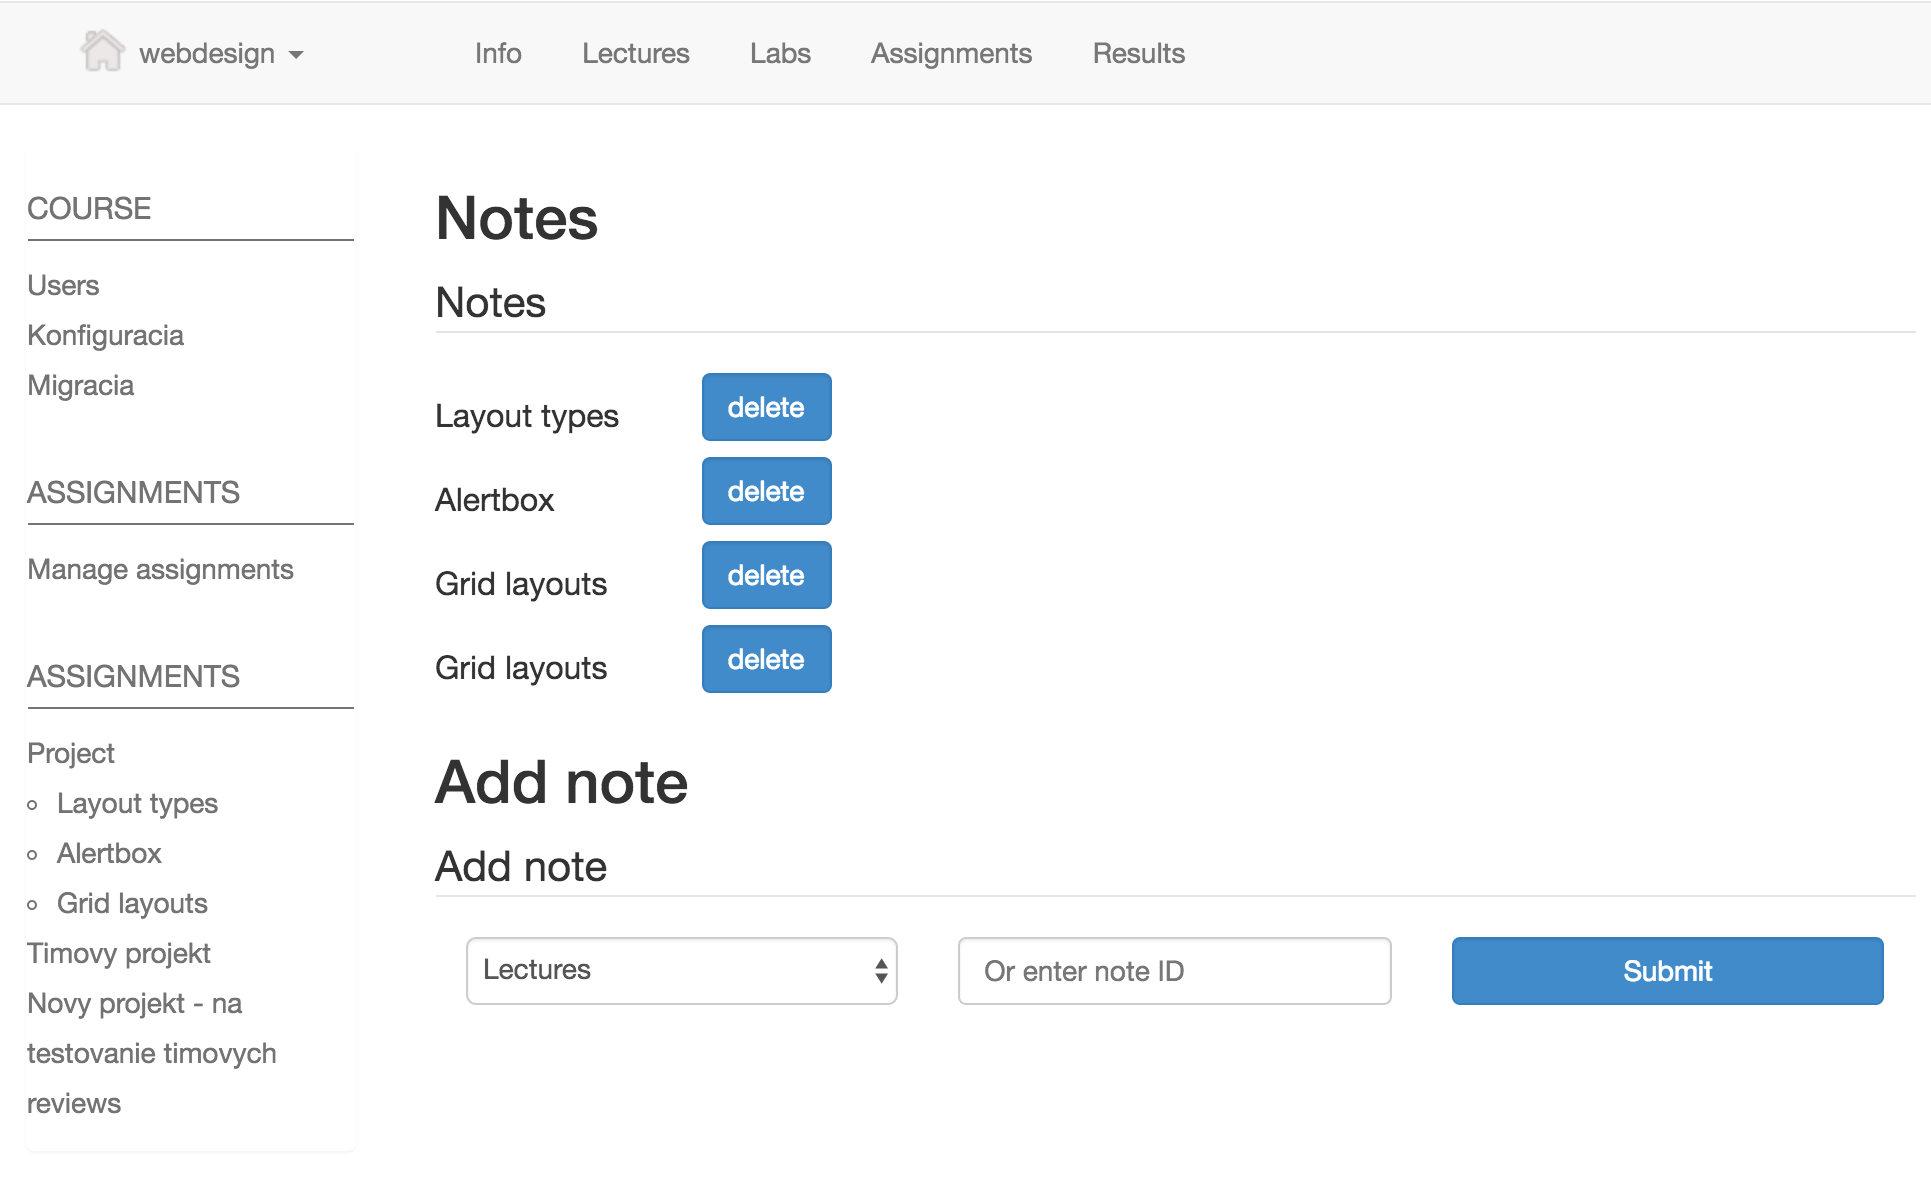
\includegraphics[width=0.9\textwidth]{images/notes.png}
    \caption{Adding notes to an assignment}
    \label{assignmentnote}
\end{figure}

\subsection{Implementation}
As seen on figure \ref{assignmentnote}, notes can be linked with an assignment and then can be shown together with it. This can be done only by a teacher in administration interface of an assignment. These notes are then showed in user dashboard. We explain this later, in the next section of these work.


For creating such connection, we altered database model and added a table \texttt{assignment\_note}, which contains many to many relationship between fields \texttt{assignment\_id} and \texttt{note\_id}. When displaying any assignment, note module is providing an interface to get any note by it's id.


\section{Assignment dashboard}

After an intense development of Assignments module, interface for submitting and viewing submissions was ambiguous and primitive. With the ability to link notes from Notes module, things started to get scattered which could confuse students. After intense brainstorming about fixing this problem, we come up with an assignment dashboard. This dashboard could offer easy access to all notes, reviews and assignments and, what could be important, could notify students about upcoming deadlines.

\begin{figure}[h]
    \centering
    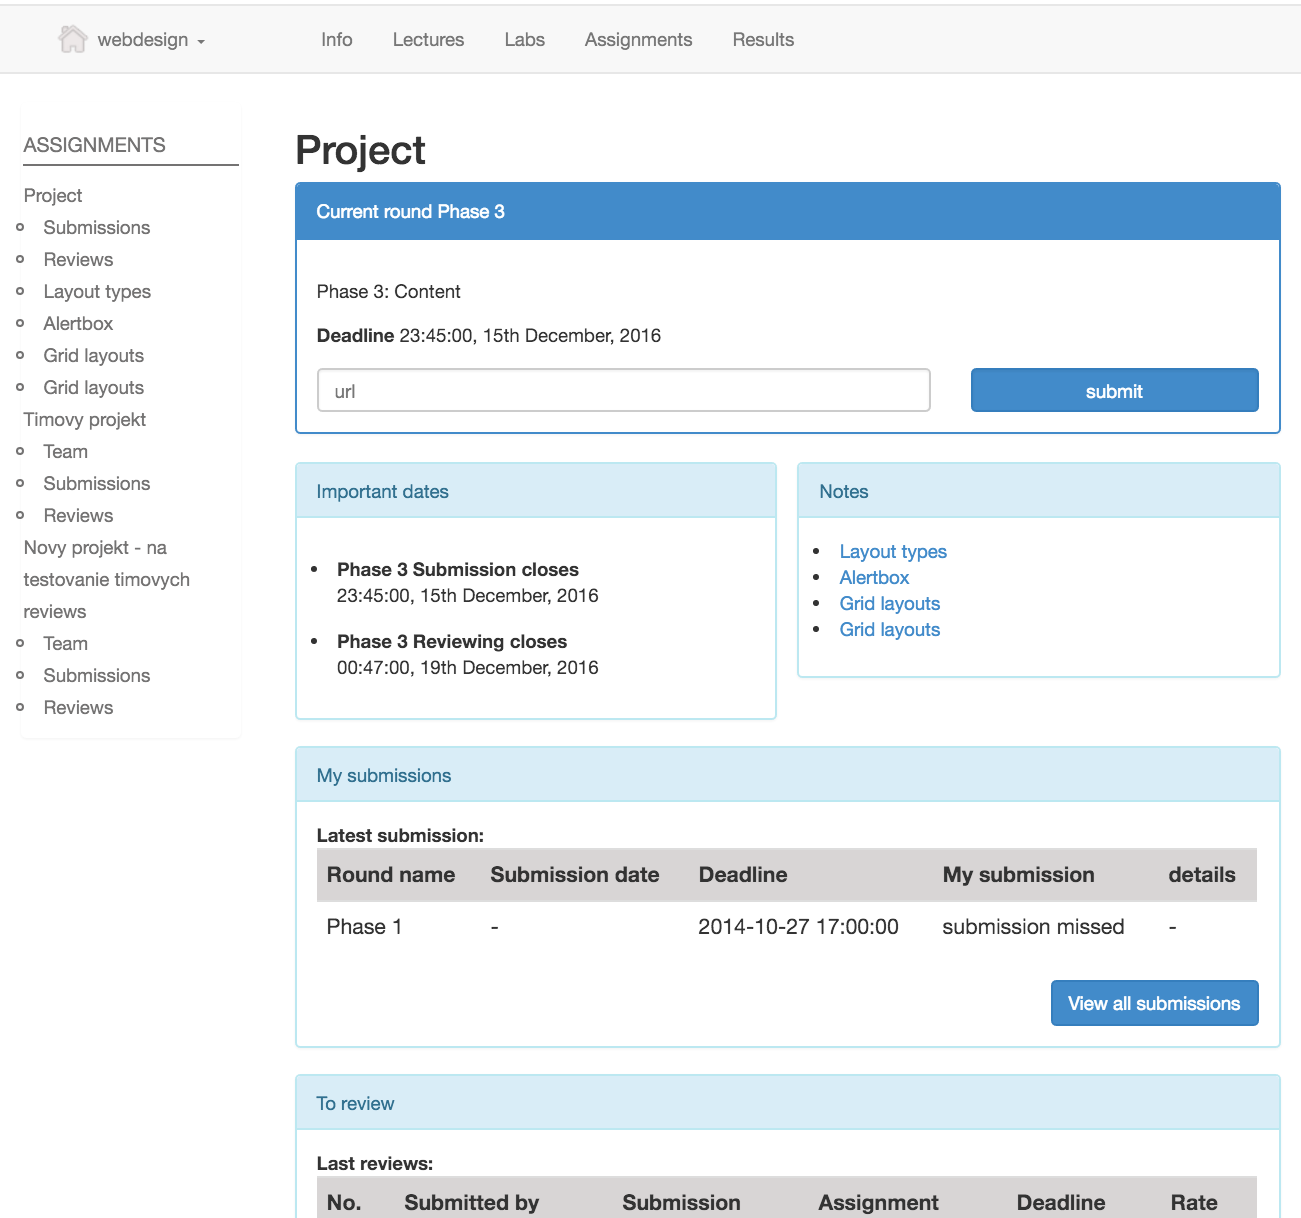
\includegraphics[width=0.9\textwidth]{images/dashboard.png}
    \caption{Assignments dashboard}
    \label{fig:assignments_dashboard}
\end{figure}

Result of our efforts is the dashboard that is shown on figure \ref{fig:assignments_dashboard}. This dashboard can be splitted into multiple sections.

First section is always showing critical information. On figure \ref{fig:assignments_dashboard} there is no critical information shown. By this, we mean mostly team forming deadlines, which must be finished until deadline and user can not submit an assignment if he has not enough team members.

First section is displaying current tasks student has to accomplish. This serves as a reminder on the top of the page and displays reviews to review or assignment rounds to submit if the user had not done it already

The next section displays important upcoming dates. There are shown 3 tasks with the closest deadline. These task may not be yet active and ready for submitting, we are just reminding students not to forget about them. 

Section labelled as Notes is showing all notes of this assignment. These notes were explained in the previous section of this work.

Next section is called My submissions. This section shows only 3 latest submissions with ability to view all submissions. These submissions are then displayed on another page. This page is also part of dashboad.

Finally, section My reviews offers similar functionality as the previous section. All reviews can also be viewed on another page.


To sum up, all information any student needs to get information about his assignments can be viewes in this dashboard. The dashboard consist of subpages which aim to provide more information about student reviews and submissions. 

\section{Bug fixing and code maintenance}
Finally, this work also included fixing many bugs found in previous versions of this system. Since Courses 2 was developed by multiple students, all separately developped parts sometimes didn't work well together so we had to find these bugs and fix them. We, however, do not consider these bugs to be important to write about.

